% fig1_pathway.tex -- where electrode coverage enters the surgical pathway.
\documentclass[tikz,border=4pt]{standalone}
% ecogstyle.tex -- colours, fonts and plot defaults shared by every figure of
% ecog_coverage.tex.  \input by each standalone figure in this directory.
%
% Colour roles (validated as one categorical palette: adjacent and all-pairs
% CVD separation >= 9, normal-vision separation >= 16; aqua sits below 3:1
% against white, so every aqua mark also carries a marker and a direct label):
%   cBlue    contacts placed by covering radius, single coverage (k = 1)
%   cOrange  the documented 8x8 subdural grid
%   cAqua    contacts restricted to gyral crowns (what a sheet can reach)
%   cViolet  contacts placed by covering radius, double coverage (k = 2)
%   cRed     cortex no contact sees; an onset zone that is missed
\usepackage{amsmath,amssymb}
\usepackage{lmodern}
\usepackage[T1]{fontenc}
\usepackage{tikz}
\usepackage{pgfplots}
\pgfplotsset{compat=1.18}
\usetikzlibrary{arrows.meta,positioning,shapes.geometric,shapes.misc,
  calc,fit,backgrounds,decorations.pathreplacing,patterns,shadows}
\usepgfplotslibrary{fillbetween,groupplots}

\definecolor{cBlue}{HTML}{2A78D6}
\definecolor{cOrange}{HTML}{EB6834}
\definecolor{cAqua}{HTML}{1BAF7A}
\definecolor{cViolet}{HTML}{4A3AA7}
\definecolor{cRed}{HTML}{E34948}
\definecolor{cInk}{HTML}{0B0B0B}
\definecolor{cInk2}{HTML}{52514E}
\definecolor{cMuted}{HTML}{8A8983}
\definecolor{cGrid}{HTML}{E4E3DF}
\definecolor{cSurface}{HTML}{FCFCFB}
\definecolor{cWash}{HTML}{F3F2EF}
\definecolor{cCortex}{HTML}{D9CFC4}
\definecolor{cCortexDark}{HTML}{9C8B7A}
\definecolor{cBlueLight}{HTML}{CDE2FB}
\definecolor{cBlueMid}{HTML}{86B6EF}

\pgfplotsset{
  ecog/.style={
    width=7.2cm, height=5.4cm,
    axis line style={cInk2, line width=0.5pt},
    tick style={cInk2, line width=0.5pt},
    major tick length=3pt,
    grid=major,
    grid style={cGrid, line width=0.4pt, solid},
    tick label style={font=\footnotesize, text=cInk2},
    label style={font=\small, text=cInk},
    title style={font=\small\bfseries, text=cInk, align=center},
    legend style={font=\footnotesize, draw=none, fill=white,
      fill opacity=0.9, text opacity=1, text=cInk,
      row sep=1pt, inner sep=2pt},
    legend cell align=left,
    every axis plot/.append style={line width=1.4pt, line join=round,
      line cap=round},
    axis background/.style={fill=white},
    clip marker paths=true,
  },
  mk/.style={mark=*, mark size=2.1pt,
    mark options={solid, draw=white, line width=0.6pt}},
  mksq/.style={mark=square*, mark size=2.0pt,
    mark options={solid, draw=white, line width=0.6pt}},
  mktri/.style={mark=triangle*, mark size=2.6pt,
    mark options={solid, draw=white, line width=0.6pt}},
  mkdia/.style={mark=diamond*, mark size=2.7pt,
    mark options={solid, draw=white, line width=0.6pt}},
}

% panel letters
\newcommand{\panel}[1]{\textbf{\sffamily (#1)}}
\tikzset{
  panellabel/.style={font=\small\bfseries\sffamily, text=cInk,
    anchor=north west, inner sep=0pt},
  note/.style={font=\footnotesize, text=cInk2, align=center},
}

\begin{document}
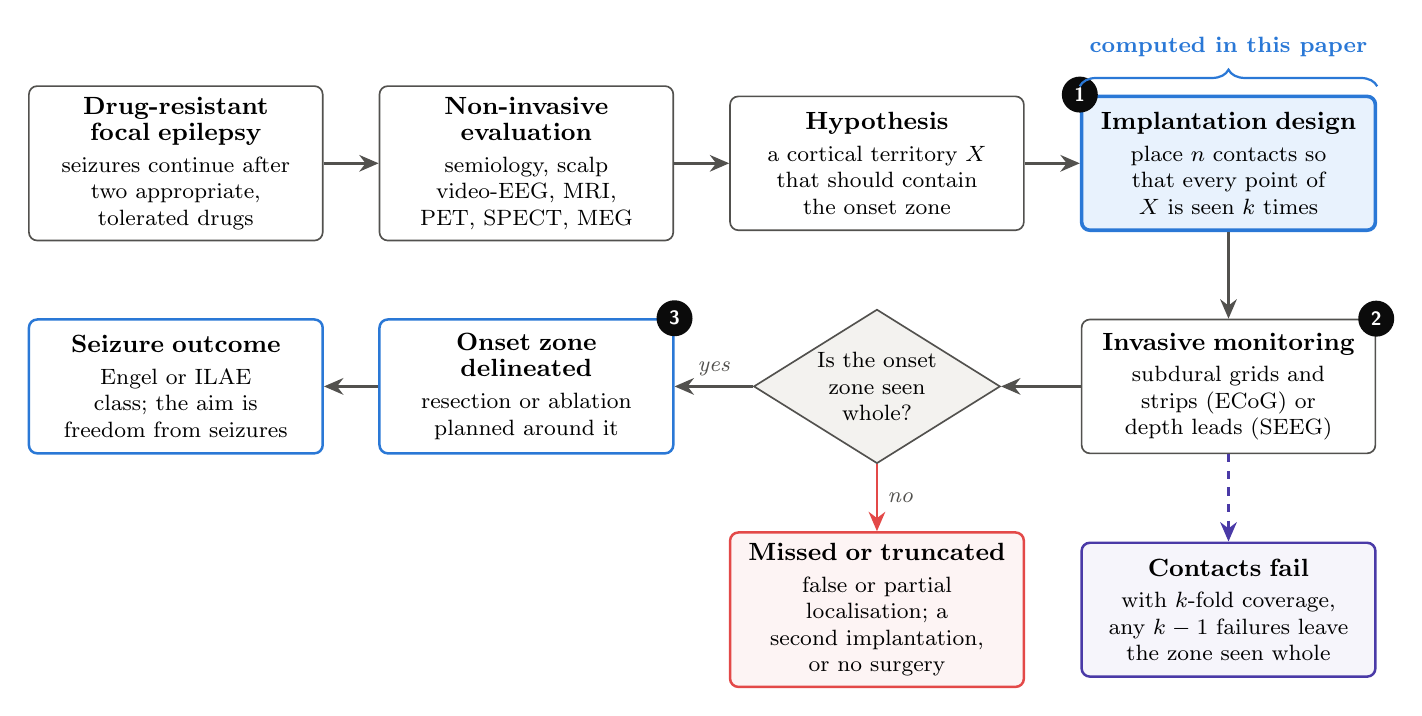
\begin{tikzpicture}[
  font=\footnotesize,
  box/.style={rectangle, rounded corners=3pt, draw=cInk2, line width=0.6pt,
    fill=white, align=center, text width=3.45cm, minimum height=1.7cm,
    inner sep=4pt, execute at begin node={\hyphenpenalty=10000}},
  focus/.style={box, draw=cBlue, line width=1.3pt, fill=cBlueLight!45},
  good/.style={box, draw=cBlue, line width=0.9pt},
  bad/.style={box, draw=cRed, line width=0.9pt, fill=cRed!6},
  dec/.style={diamond, aspect=1.6, draw=cInk2, line width=0.6pt, fill=cWash,
    align=center, inner sep=0pt, text width=1.75cm},
  flow/.style={-{Stealth[length=7pt,width=6pt]}, line width=1.0pt, color=cInk2},
  lab/.style={font=\footnotesize\itshape, text=cInk2},
  hd/.style={font=\small\bfseries},
  stepno/.style={circle, fill=cInk, text=white, font=\scriptsize\bfseries\sffamily,
    inner sep=1.3pt, minimum size=13pt},
]
% ---------------------------------------------------------------- row 1
\node[box] (dre) {{\small\bfseries Drug-resistant focal epilepsy}\\[2pt]
  seizures continue after two appropriate, tolerated drugs};
\node[box, right=0.7cm of dre] (noninv) {{\small\bfseries Non-invasive evaluation}\\[2pt]
  semiology, scalp video-EEG, MRI, PET, SPECT, MEG};
\node[box, right=0.7cm of noninv] (hyp) {{\small\bfseries Hypothesis}\\[2pt]
  a cortical territory $X$ that should contain the onset zone};
\node[focus, right=0.7cm of hyp] (design) {{\small\bfseries Implantation design}\\[2pt]
  place $n$ contacts so that every point of $X$ is seen $k$ times};
% ---------------------------------------------------------------- row 2
\node[box, below=1.1cm of design] (monitor) {{\small\bfseries Invasive monitoring}\\[2pt]
  subdural grids and strips (ECoG) or depth leads (SEEG)};
\node[dec] (seen) at (hyp |- monitor) {Is the onset zone seen whole?};
\node[good] (loc) at (noninv |- monitor) {{\small\bfseries Onset zone delineated}\\[2pt]
  resection or ablation planned around it};
\node[good] (outcome) at (dre |- monitor) {{\small\bfseries Seizure outcome}\\[2pt]
  Engel or ILAE class; the aim is freedom from seizures};
% ---------------------------------------------------------------- row 3
\node[bad, below=0.85cm of seen] (miss) {{\small\bfseries Missed or truncated}\\[2pt]
  false or partial localisation; a second implantation, or no surgery};
\node[box, draw=cViolet, line width=0.9pt, fill=cViolet!5]
  (fail) at (monitor |- miss) {{\small\bfseries Contacts fail}\\[2pt]
  with $k$-fold coverage, any $k-1$ failures leave the zone seen whole};
% ---------------------------------------------------------------- arrows
\draw[flow] (dre) -- (noninv);
\draw[flow] (noninv) -- (hyp);
\draw[flow] (hyp) -- (design);
\draw[flow] (design) -- (monitor);
\draw[flow] (monitor) -- (seen);
\draw[flow] (seen) -- node[lab, above] {yes} (loc);
\draw[flow, cRed] (seen) -- node[lab, right] {no} (miss);
\draw[flow] (loc) -- (outcome);
\draw[flow, dashed, cViolet] (monitor) -- (fail);
% steps
\node[stepno] at (design.north west) {1};
\node[stepno] at (monitor.north east) {2};
\node[stepno] at (loc.north east) {3};
% brace over the part this paper computes
\draw[decorate, decoration={brace, amplitude=6pt, raise=3pt}, line width=0.8pt, cBlue]
  (design.north west) -- (design.north east)
  node[midway, above=10pt, font=\footnotesize\bfseries, text=cBlue] {computed in this paper};
\end{tikzpicture}
\end{document}
